Throughout the project, we have developed in total 3 sub-projects;
\begin{itemize}
\item Angular2-interface: Our graphic user interface
\item music-streamer-library: A library utilized by our interface
\item fake-dht: A fake implementation of a \acs{DHT} network
\end{itemize}
Below is a list of contributions to each of these projects, by group member;
As the lists contain aliases, we provide a mapping below:
\begin{itemize}
    \item Skeen $\Rightarrow$ Emil Madsen (20105376)
    \item RasmusMJ $\Rightarrow$ Rasmus Mosbech Jensen (20105109)
    \item MortenSoerensen $\Rightarrow$ Morten Kryger Sørensen (20118128)
\end{itemize}

\section{Angular2-interface}
This repository contains our web-interface implemented using Angular2 (also 
known as Angular.io), this interface was developed during the Angular-Attack
hackathon event (May 14-15).
\newline\newline
% TODO: Update LOC
The repository contains 2477 lines of code, at hand-in time, and has undergone 
several refactoring during and after the hackathon.

\begin{figure}[H]
  \centering
    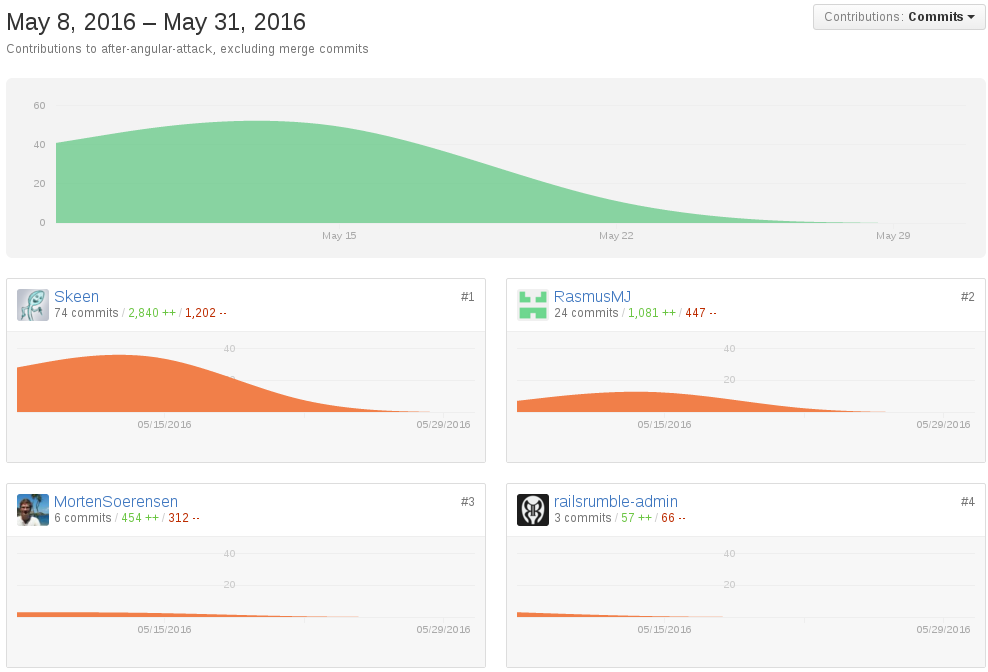
\includegraphics[width=\linewidth]{gfx/Angular-interface}
  \caption{A graph from GitHub laying out contributions by group members. - Angular2-interface}
  \label{fig:angular-interface}
\end{figure}

\section{music-streamer-library}
\label{sec:appendix-music-streamer-library}
This repository contains our library, which underlies our Angular2-interface,
the motivation for splitting the project, is that the library can be utilized 
by multiple interfaces or clients, as we originally intended to develop both a
web-interface client and a node.js client.
\newline\newline
% TODO: Update LOC
To version of the library exists; the stripped version and the unstripped
version. The stripped version contains 949 lines of code, at hand-in time, while
the unstripped version contains 1942 lines of code.

\begin{figure}[H]
  \centering
    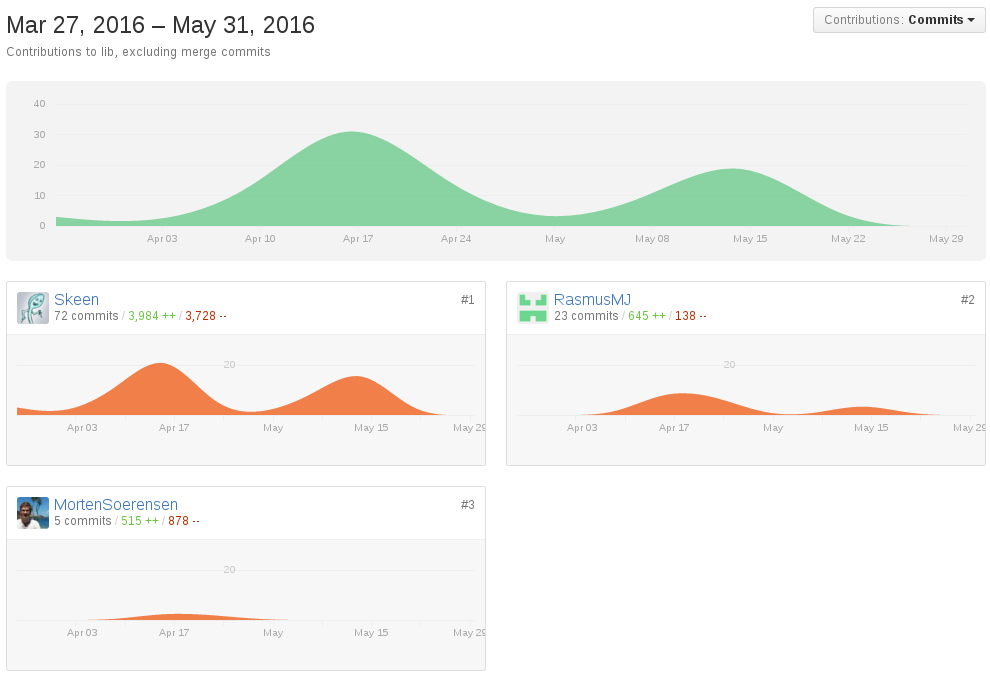
\includegraphics[width=\linewidth]{gfx/Music-streamer-library}
    \caption{A graph from GitHub laying out contributions by group members. - Music-streamer-library (stripped version)}
  \label{fig:music-stramer-library}
\end{figure}

\section{fake-dht}
This repository contains our faked \acs{DHT} implementation, which fulfills the \acs{DHT}
interface within our music-streamer-library by utilizing a centralized server.
\newline
Two different version have been developed, one which fakes a traditional \acs{DHT}
and one which fakes a \acs{PHT} running on top of a \acs{DHT}.
\newline\newline
% TODO: Update LOC
The \acs{DHT} fake contains 101 lines of code, at hand-in time, while the \acs{PHT} fake 
contains 99 lines of code. The two versions utilize different libraries.

\begin{figure}[H]
  \centering
    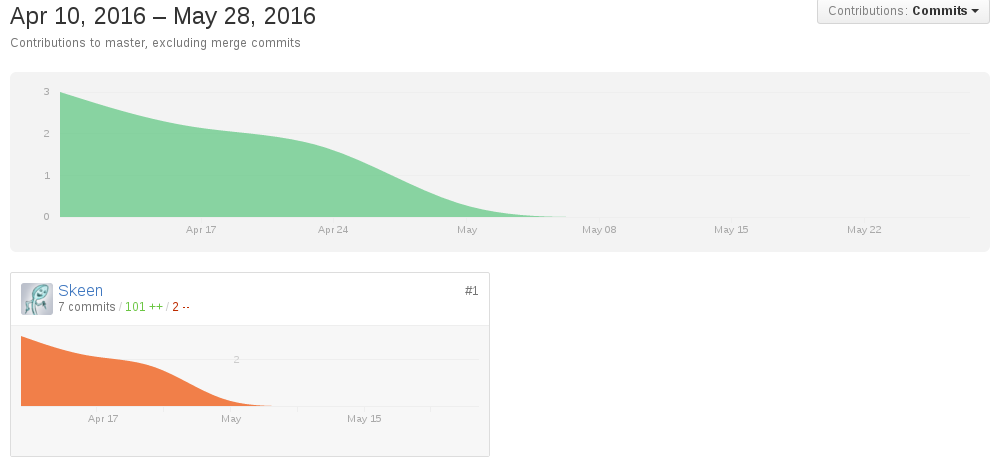
\includegraphics[width=\linewidth]{gfx/dht-fake}
    \caption{A graph from GitHub laying out contributions by group members. - dht-fake}
  \label{fig:music-stramer-library}
\end{figure}

\begin{figure}[H]
  \centering
    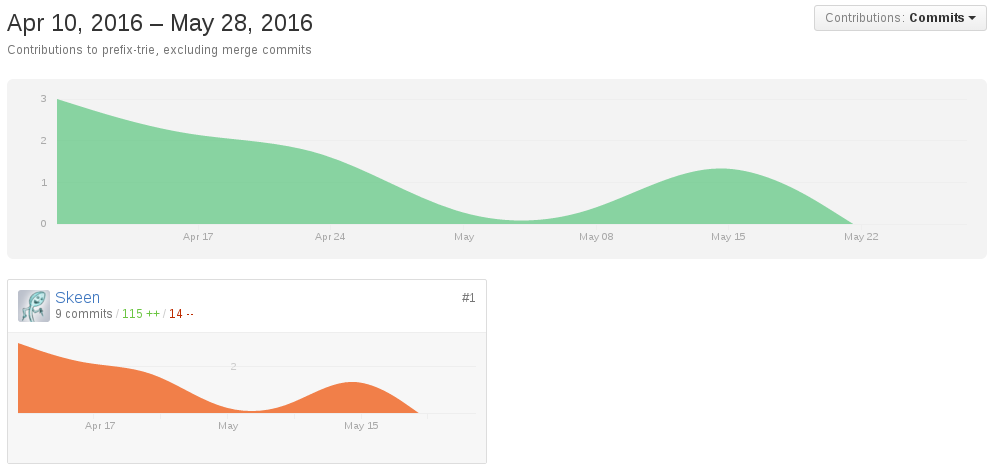
\includegraphics[width=\linewidth]{gfx/pht-fake}
    \caption{A graph from GitHub laying out contributions by group members. - pht-fake}
  \label{fig:music-stramer-library}
\end{figure}

\section{Other contributions}
In addition to these contributions, we've made several pull requests for the
libraries we depend on; namely to:
\begin{itemize}
\item music-metadata: A library to parse out meta-data from music files.
\item Kad-WebRTC: A transportation layer for the 'Kad' Kademlia implementation.
\item localforage: A unified interface library for persistent browser-storage
    technologies.
\item electron-eval: A library to execute code within a headless browser
    (electron).
\end{itemize}

Below is a list of contributions to each of these projects, by group member:
\subsection{music-metadata}
A pull request and a bug report has been submitted.

\subsubsection{General data stream support}
A \href{https://github.com/leetreveil/musicmetadata/pull/114}{pull request} to
add support for general data streams (not just npm-stream) has been submitted
to the upstream developer: the patch adds 40 lines of code, and removes 40
lines of code.
\newline\newline
The patch was created and submitted by Emil Madsen, and has been rejected by
the upstream developer, whom has implemented the suggested feature in another
way. The newest version of the music-metadata library contains this update.

\subsubsection{Bug report regarding invalid stream usage}
A \href{https://github.com/leetreveil/musicmetadata/pull/116}{pull request} to
add support for stopping read steams as soon as meta-data has been emitted was
accepted into the upstream library.

The content of this pull request did however misuse streams, in a way which is
generally not supported, as such the acceptance of this pull request broke our
code.

Group member Emil Madsen reported this issue to the upstream developer in a
\href{https://github.com/leetreveil/musicmetadata/issues/120}{bug report},
after which the pull request was reverted.

\subsection{Kad-WebRTC}
\label{subsec:appendix-kad-webrtc}
While experimenting with 'Kad-WebRTC' we ran the provided examples, 
unfortunately all of these ran within the same browser tab, and as such we were
not convinced that the library would work across multiple browsers (or tabs).

In order to confirm the operability of the library under these circumstances,
we developed an interactive example, which has been submitted as a 
\href{https://github.com/kadtools/kad-webrtc/pull/11}{pull request}. This pull
request adds 181 lines of code and removes 5.
\newline\newline
The example was created and submitted by Emil Madsen, and has been accepted by
the upstream developer, after a bit of ping-pong regarding the details of the 
pull request.

\subsection{localforage}
\label{subsec:appendix-localforage}
A \href{https://github.com/mozilla/localForage/pull/551}{pull request} to add 
node.js support to the Mozilla project localforage (A unified interface for 
the browser-based persistent storage technologies) has been submitted to the
upstream developers: the patch adds 5664 lines of code (of which 5001 are 
generated by the built system), as such 663 lines of code has been written.
Additionally 3 lines of code has been removed.
\newline\newline
The patch was created and submitted by Emil Madsen, the pull request is still
open, and unlikely to be merged in it's current state. The upstream developers
like the concept and idea presented by the pull request, but cannot accept it,
due to the quality of the utilized libraries.

The created patch do however fulfill our own use-case; that is to enable us to 
develop a proof-of-concept 'node.js' client using our music-streamer-library
(which in turn utilizes localforage for persistent storage).

\subsection{electron-eval}
\label{subsec:appendix-electron-eval}
A \href{https://github.com/mappum/electron-eval/issues/29}{bug report} and 
debugging assistance been provided to the upstream developer, to get the project
running in headless Linux environments (docker for our use-case).
\newline\newline
As a part of this process, several docker images has been created and shared
with the upstream developer, whom has patched the library. This patch combined
with a mapping of the missing external dependencies, has resulted in a
successful recipe for running the project in a headless Linux setting.

The upstream developer considers patching the library further to ease future 
debugging of missing external dependencies. A duplicate of this issue has been
reported to WebTorrent, which was the original blocker for our application.
\newline\newline
The bug report, and the subsequent debugging assistance provided to the
upstream developer was by Emil Madsen.

